\section{Experimental Evaluation}
\label{section:experiment}
To evaluate our prototype~\toolname, we conducted a detailed experimental evaluation on the available MUS benchmarks.
The objective of the experimental evaluation is to evaluate the performance of \toolname~with the existing MUS enumerators.

\subsection{Benchmark and Baseline}
We collected our benchmark from two areas:~(i)~MUS track of the SAT $2011$ competition~(ii)~scalable benchmark\footnote{\url{https://gitlab.com/satisfiability/scalablesat}} 
from MUS counting~\cite{BM2020}. We compare our prototype with three MUS enumeration tools: 
~(i)~\marco~\cite{LPMM2016}~(ii)~\unimus~\cite{BC2020}~and~(iii)~\remus~\cite{BCB2018}.

\subsection{Environmental Settings}
All experiments were conducted on a high-performance computing cluster equipped with nodes featuring AMD EPYC $7713$ CPUs, each with $128$ real cores. 
%We imposed a runtime limit of 5000 seconds and a memory cap of 16GB for each experiment.
%All experiments were carried out on a high-performance computer cluster, where each node consists of AMD EPYC $7713$ CPUs running with $128$ real cores. 
Throughout the experiment, the runtime and memory limits were set to $3600$ seconds and $16$GB, respectively, for all considered tools.

\subsection{Experimental Result}
We present the performance of all MUS enumerators in~\Cref{table:mus_enumeration_result}.
To compare the performance, the table shows the number of solveds instances of all MUS enumerators and their corresponding PAR-$2$ scores.
An instance is considered to be solved by a tool if the tool is able to enumerate all of its MUSes. 
The table clearly demonstrates that \toolname~outperforms existing MUS enumerators.
\begin{table}[h]
    \centering
    \begin{tabular}{m{5em} m{3em} m{3em} m{3em} m{5em}} 
    \toprule
    % & & \rotatebox{60}{\clingo} & \rotatebox{60}{DynASP} & \rotatebox{60}{Ganak}  & \rotatebox{60}{ApproxMC} & \rotatebox{60}{ApproxASP} \\ 
     & \marco & \unimus & \remus & \toolname\\
    \midrule
    \#Solved ($983$) & 248 & 248 & 245 & 547\\
    \midrule
    PAR-$2$ & 5422 & 5417 & 5441 & 3226\\
    \bottomrule
    \end{tabular}
    \caption{The performance of \toolname~vis-a-vis different MUS solvers.}
    \label{table:mus_enumeration_result}
\end{table}
\begin{figure}
    \centering
    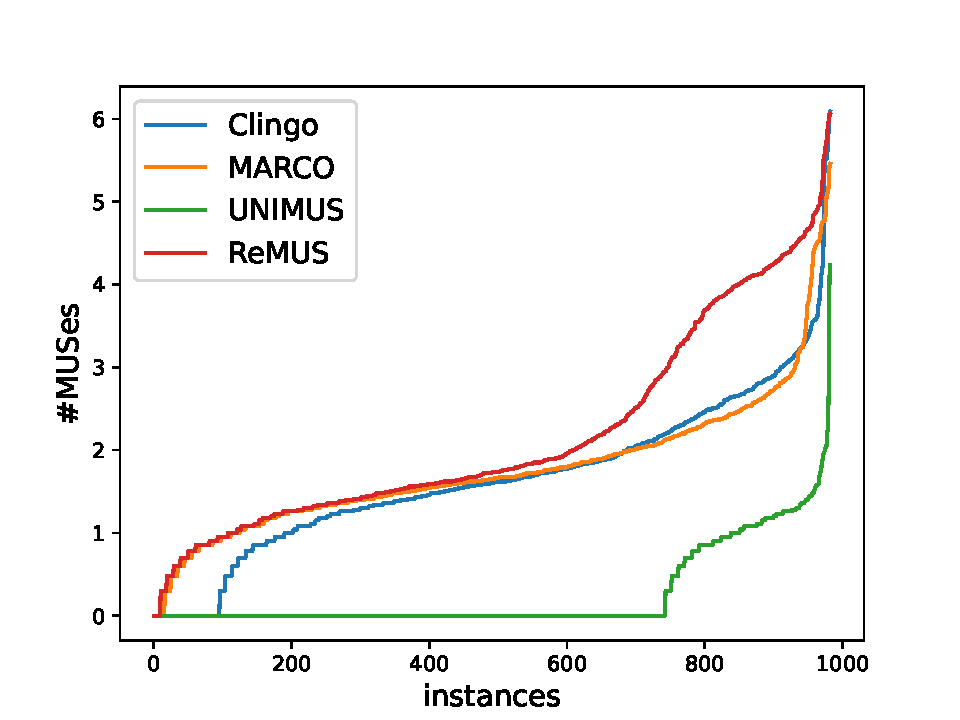
\includegraphics[scale=0.5]{images/countMUS.pdf}
    \caption{The number of MUSes enumerated by \toolname~by vis-a-vis other enumerators.}
    \label{fig:number_of_mus}
\end{figure}

